\subsection{The micro-service model}
%Microservice architecture
Implementing a complete monolithic architecture was seen as an unreliable and inconvenient solution for the nature of our problem. Besides the fact that many enterprises have started to shift from monolithic to micro-service architecture, considering the many benefits that the later has compared to the former, one of the reason we decided to use a micro-service architectural style is the loose-coupling of components. Ceccarelli et al. \cite{3} supports the idea that for an entity linking process a unique framework is shared where the recognition, disambiguation and linking processes are well separated and easy to isolate in order to study their performance. Therefore, a microservice architecture is best fit for our case. According to Lewis and Fowler \cite{martinfowler}, a microservice architectural style is an approach for developing a complete application as a suite of small services, which are executed individually, each on its own process and communicate with each other using lightweight mechanisms, usually over HTTP. Implementing our framework in such a way allows us to follow a more generic and abstract approach to \ac{ned} since the different modules composing the framework can be easily changed to fit for other \ac{nlp} tasks such as \ac{wsd}, co-reference resolution or even changing the language of the task to something other than English. Illustrated in Figure \ref{fig:microservice_architecture}, our framework is composed of 7 different microservices loosely coupled from each other with various responsibilities that build up the complete solution to the \ac{ned} problem.
\newpage 

\begin{figure}[]
  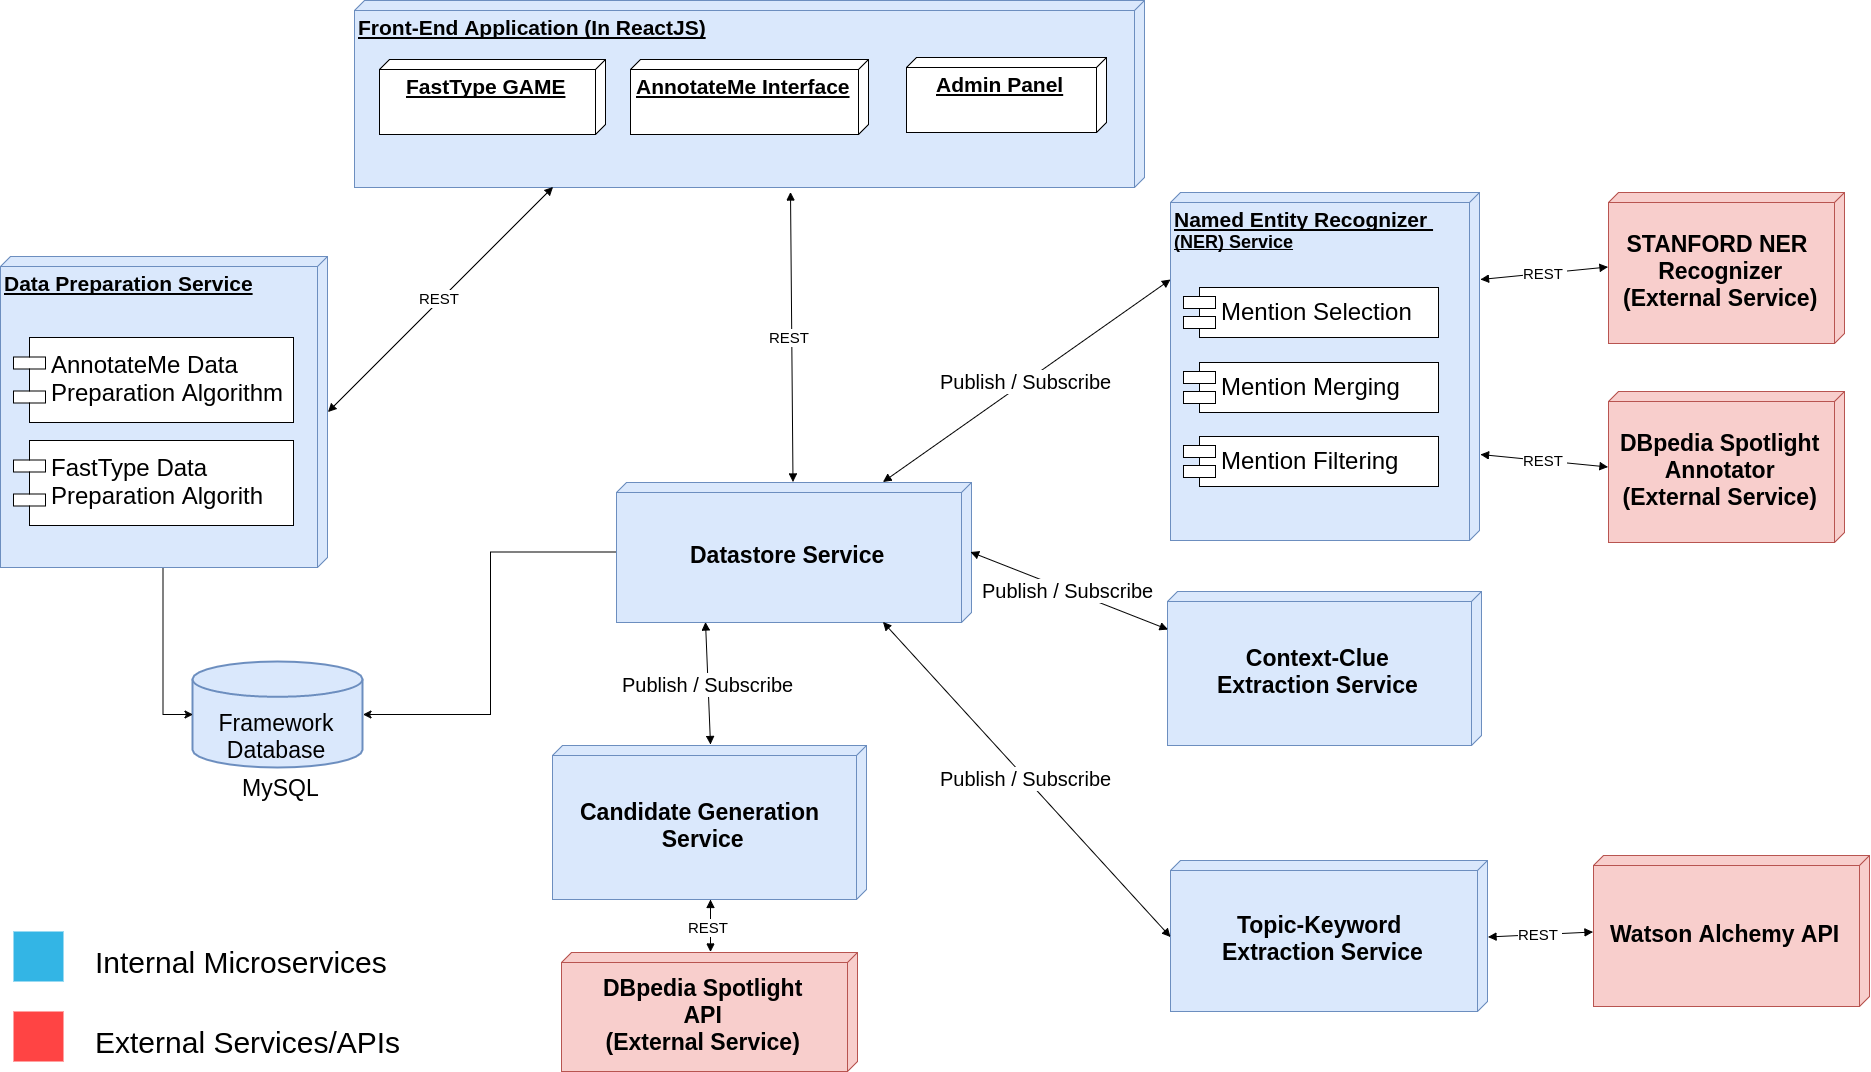
\includegraphics[width=\linewidth]{figures/microservice-architecture.png}
  \caption{Overview of the NED micro-service architecture}
  \label{fig:microservice_architecture}
\end{figure}

Observing the figure above, two different categories can be identified. The internal microservices (boxes highlighted with blue) are services that have been completely implemented from scratch. On the other hand, the external microservices (boxes highlighted in red) are external open source services that have been used by our framework to perform actions which were out of scope of this study. Among the external services, \textit{Stanford NER Recognizer} was the only external service that was not available as an online service offering API calls to perform the corresponding actions. A detailed explanation of the NER microservice is provided later in section \ref{framework:architecture_NER}.

%Communication Infrastructure
In a microservice architecture, a key factor that differs this architecture from other design patterns is the lightweight communication/messaging infrastructure. In our framework, we have utilized two different communication protocols, namely, Synchronous Messaging (\ac{rest}) and Asynchronous Messaging (\ac{amqp}). In cases where immediate response is required from a service to another, RESTful request/response API calls have been used to exchange information. We have tried to adhere to the fundamental rules of the RESTful messaging protocols where every functionality of the service is represented with a resource and operations carried out on top of these resources. As illustrated in Figure \ref{fig:microservice_architecture}, the front-end service which contains the admin panel, AnnotateMe Interface and Fastype Game communicate synchronously with the data preparation service and data store service. In addition to the front-end service, all external services are invoked using synchronous REST API calls since our internal microservices are not able to perform any internal actions unless the response from the external service is acquired. A complete documentation of the REST API calls implemented in the data store and data preparation services are available in Appendix \ref{appendix1:RESTDOCsec}.

Some of the services that compose the framework usually have a longer processing time compared to others because of the underlying complexity and the calculations that need to be performed. In these cases, it is more practical to use asynchronous messaging protocols without having to freeze the overall process as a consequence of one service which takes longer to complete. The publish and subscribe asynchronous message communication model was used for this purpose. More specifically, RabbitMQ \footnote{RabbitMQ Documentation Page \url{https://www.rabbitmq.com/documentation.html}} was used as the underlying lightweight message brooker based on \ac{amqp} (Advanced Message Queue Protocol). To see the different publishing and subscription routes that build the asynchronous communication infrastructure of the framework, see Appendix \ref{appendix1:AMQPDOCsec}.

%Conteinarization - Docker 
When designing a microservice architecture, among the many important design patterns that distinguish this architectural style from others is the deployment process. The deployment of microservices plays a critical role and when it comes to microservice architecture, the following key requirements have to be satisfied \cite{dzone}:
\begin{itemize}
    \item The ability to deploy/un-deploy independently each service
    \item It must be able to scale at each microservice level (as some services may experience more trafic than others)
    \item The ability to build and deploy microservices quickly
    \item In case one microservice fails to execute, other microservices should not be affected by this failure
\end{itemize}

To comply with the above mentioned requirements, Docker\footnote{Docker Documentation Page \url{https://docs.docker.com/}} was considered as the best microservice deployment solution. Docker is a containerization tool that lets developers and system administrators deploy self-sufficient application containers in Linux environments \cite{dzone}. Deploying a microservice into a docker container is as easy as writing a 5 line script. The steps involved to deploy an application into a docker container are as follows \cite{dzone}: 
\begin{itemize}
    \item Packaging the microservice as a Docker container image (usually by writing a script)
    \item Deploying each service instance as a container
    \item Linking containers with each other so that they are able to communicate (this is done automatically by Docker)
    \item Scaling is done by deploying many instances of the same container
    \item Building, deploying and starting a microservice is relatively fast as Docker uses containers instead of virtual machines (which is much slower compared to containers)
\end{itemize}

%Technology Stack - NodeJS, ReactJS, Mysql db
In terms of technology stack used to implement the microservice framework, the latest web technology tools have been utilized. In addition to the previously mentioned tools used for communication and deployment, the actual microservice applications framework has been implemented using NodeJS\footnote{NodeJS \url{https://nodejs.org/en/docs/}} as a back-end programming language, whereas for the front-end implementation we used ReactJS\footnote{ReactJS \url{https://facebook.github.io/react/}}. The combination of NodeJs and ReactJS has proven to be very efficient in terms of development speed, performance, agile development support and the incredible fast rendering capabilities which is very helpful during development and debugging of the application. As for the data storage, MySQL relational database has been used in our framework. 

Figure \ref{fig:workflow} illustrates the complete workflow of the framework. We use this illustration as a reference when describing the different services composing the framework in the following sections.


\begin{figure}[]
  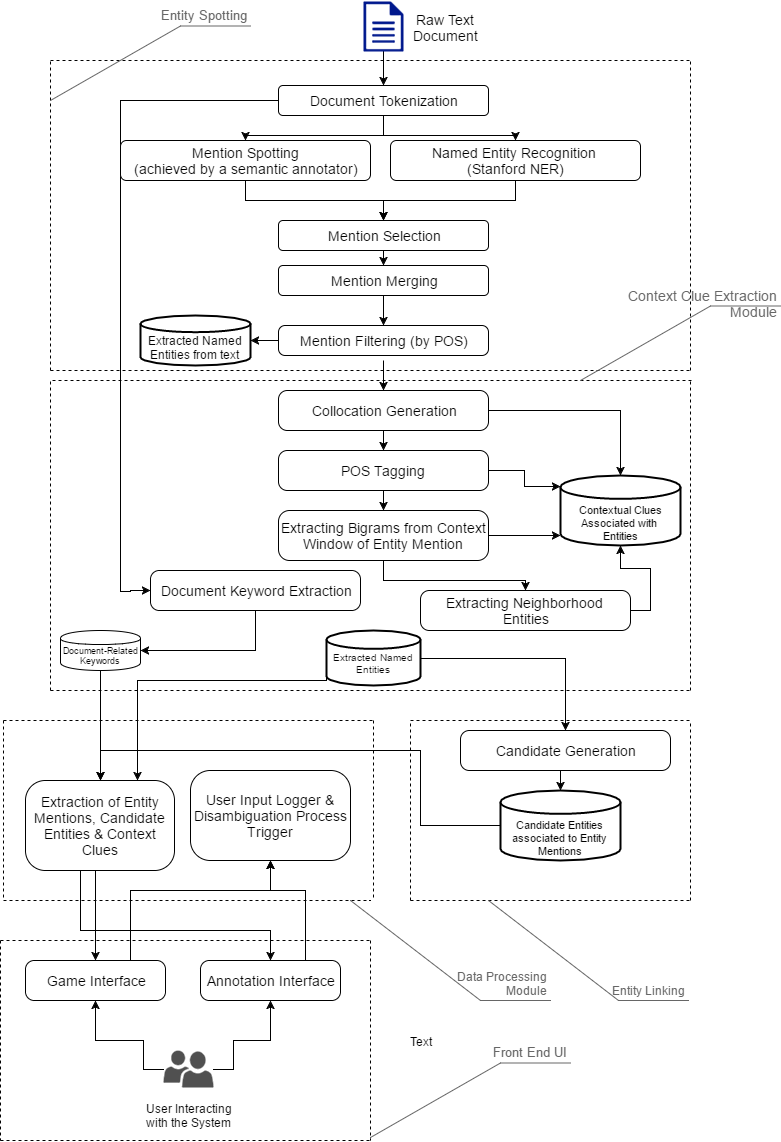
\includegraphics[width=\linewidth]{figures/workflow-diagram-v4.png}
  \caption{Overview of the complete workflow of the NED Framework}
  \label{fig:workflow}
\end{figure}
